\documentclass[11pt,a4paper]{article}

% ======================================================================
%  The Rate Inheritance Principle — Version 2 (July 2026)
%  v1: December 2025 (ai.viXra:2512.0072v1).
%  Changes (Appendix A): surrogate decay-curve evidence of v1 (uncontrolled
%  proxy class, broken figure placeholder) withdrawn and replaced by the
%  exact evidence of 2512.0064 v2; weak form promoted to a proved lemma;
%  strong form updated (derived in the quasi-free local-sink class with the
%  squared-amplitude exponent v1 anticipated; Davies-class failure realized
%  in 2512.0070 v2); secular delocalization added to the failure modes;
%  proxy-validation requirement added to the falsification protocol;
%  maintenance inequality re-anchored to 2512.0061 v2.
% ======================================================================

\usepackage[utf8]{inputenc}
\usepackage[T1]{fontenc}
\usepackage{amsmath,amssymb,amsthm,mathtools}
\usepackage[margin=1.05in]{geometry}
\usepackage{graphicx}
\usepackage[colorlinks=true,linkcolor=blue,citecolor=blue,urlcolor=blue]{hyperref}

\theoremstyle{plain}
\newtheorem{theorem}{Theorem}[section]
\newtheorem{lemma}[theorem]{Lemma}
\newtheorem{hypothesis}[theorem]{Hypothesis}
\newtheorem{conjecture}[theorem]{Conjecture}
\theoremstyle{definition}
\newtheorem{definition}[theorem]{Definition}
\theoremstyle{remark}
\newtheorem{remark}[theorem]{Remark}

\newcommand{\Tr}{\operatorname{Tr}}
\newcommand{\kB}{k_{\mathrm{B}}}
\newcommand{\eps}{\epsilon}

\title{The Rate Inheritance Principle:\\
From Static Correlations to Dynamical Decoherence Rates}
\author{Lluis Eriksson\\ \small Independent Researcher\\
\small \texttt{lluiseriksson@gmail.com}}
\date{July 4, 2026 \quad (v2; v1: December 2025) \quad ai.viXra:2512.0072}

\begin{document}

\maketitle

\begin{center}
\fbox{\parbox{0.92\textwidth}{\small
\textbf{Editorial status: companion note.} Theoretical framing note (RIP) of
the coherence-maintenance series. The exact rate-inheritance law is
ai.viXra:2512.0064 (v2) \cite{HCut}; the Davies-class stress test is
ai.viXra:2512.0070 (v2) \cite{Stress}; the work theorem is ai.viXra:2512.0061
(v2) \cite{MaintWork}; the closure map is ai.viXra:2512.0071 (v2)
\cite{Closure}. All papers, verification scripts, and reference logs are
distributed in a single companion repository; this note's figure script lives
in \texttt{verification/0072}.}}
\end{center}

\begin{abstract}
In gapped open quantum systems with localized couplings, static correlations
across an operational interface of width $\eps$ are exponentially suppressed
by the mass gap. Independently, the energetic cost of maintaining quantum
coherence is governed by the rate at which coherence is lost under
uncontrolled dynamics. The Rate Inheritance Principle (RIP) is the hypothesis
connecting the two: effective coherence-loss rates inherit the suppression
envelope of static correlations across the interface. We distinguish a weak
upper-envelope form --- stated here as a short proved lemma under explicit
integrability hypotheses --- from a stronger envelope-class conjecture, and we
record what is now known: the strong form is \emph{derived, with a
frequency-resolved exponent, in an exactly solvable quasi-free local-sink
class}, where the rate inherits the \emph{square} of the static amplitude
envelope, $\kappa(\eps) \propto e^{-2q(\omega_b)\eps}$ --- confirming the
squared-envelope caveat anticipated in v1 --- and it \emph{fails through
near-zero-frequency channels within the secular Davies model class}, whose
delocalized jump operators sustain a persistent rate floor. Version 1's
surrogate decay-curve evidence is withdrawn: it belonged to the uncontrolled
proxy class whose failure mode was exposed by the critical-point control of
the companion paper, and it is replaced here by the exact Liouvillian-rapidity
evidence. Failure modes (now including secular delocalization), a
proxy-validated falsification protocol, and the conditional operational
consequences for the quantum--classical resource boundary are stated with
explicit scope.
\end{abstract}

\section{Preliminaries and definitions}

We consider a finite-dimensional quantum system with Hamiltonian
$H_S = \sum_n E_n \Pi_n$ undergoing uncontrolled Markovian evolution generated
by a Lindbladian $\mathcal{L}_\eps$. Logarithms are natural (nats).

\textbf{Energy pinching.} $\Delta[\rho] := \sum_n \Pi_n \rho \Pi_n$.

\textbf{Coherence functional.} For faithful states $\rho$ (or with the
standard support convention),
$C(\rho) := S(\rho\|\Delta[\rho])$, with
$S(\rho\|\sigma) := \Tr[\rho(\log\rho - \log\sigma)]$.

\textbf{Coherence-loss rate.} For $\rho_t = e^{t\mathcal{L}_\eps}(\rho)$,
$\dot{C}_{\mathrm{loss}}(\rho) := -\frac{d}{dt}C(\rho_t)\big|_{t=0}$.

\textbf{Weak-coherence regime.} A family of states lies in the weak-coherence
regime if for every $\delta > 0$ there exists $C_0(\delta) > 0$ such that
$C(\rho) \le C_0(\delta)$ implies
$|\dot{C}_{\mathrm{loss}}(\rho) - \kappa(\eps)\,C(\rho)| \le \delta\,C(\rho)$,
uniformly over the family. (This is a \emph{two-sided} rate-proportionality
assumption: it asserts that the channel with rate $\kappa(\eps)$ is the one
actually seen by the states of interest. The ceiling/floor distinction of
\cite{Stress} (v2) makes precise what can go wrong when it is dropped.)

\section{The missing dynamical bridge}

Static clustering in gapped systems and thermodynamic lower bounds on
coherence maintenance are independently established. Static correlators
across an interface of width $\eps$ obey bounds of the form
\begin{equation}
\text{correlations} \;\lesssim\; f(\eps), \qquad
f(\eps) \sim \mathrm{poly}(m\eps)\, e^{-m\eps} \;\text{or}\; K_\nu(m\eps),
\end{equation}
with the lattice and continuum instances developed in \cite{Clustering}.
Independently, maintenance costs satisfy
$P_{\mathrm{extra}}(\rho) \ge \kB T\, \dot{C}_{\mathrm{loss}}(\rho)$ under an
explicit operational control model --- in the corrected form of
\cite{MaintWork} (v2): unconditionally for the total power via the entropy
production rate; against thermodynamically efficient population baselines for
the extra power; and with no further assumptions when the pinched target is
stationary (pure dephasing), the case relevant below. What remains is how the
effective rate $\kappa(\eps)$ depends on $\eps$. RIP isolates this step.

\section{The Rate Inheritance Principle}

\subsection{Effective coherence-loss rate}

We define the effective rate as an envelope over microscopic Davies rates,
\begin{equation}
\kappa(\eps) := \max_\omega \|\Gamma(\omega; \eps)\|,
\end{equation}
where $\Gamma(\omega;\eps) = [\Gamma_{\alpha\beta}(\omega;\eps)]$ is the
Hermitian Kossakowski matrix at Bohr frequency $\omega$.

\begin{remark}[This is a ceiling]\label{rem:ceiling}
$\kappa(\eps)$ bounds the fastest channel. Upper-envelope statements
(Lemma~\ref{lem:weak}) are therefore statements about $\kappa$; conclusions
about maintenance \emph{costs} additionally need the two-sided weak-coherence
regime above, or a floor envelope in the sense of \cite{Stress} (v2). v1 did
not draw this distinction; the series now does, and this note inherits it.
\end{remark}

\subsection{Weak form (upper envelope): a lemma}

\begin{lemma}[Rate inheritance, weak form]\label{lem:weak}
Let the Davies rates be
$\Gamma_{\alpha\beta}(\omega;\eps) = \int_{-\infty}^{\infty} dt\, e^{i\omega t}
\langle B_\alpha(t;\eps) B_\beta(0;\eps)\rangle$, where $B_\alpha(\cdot;\eps)$
enters a system--bath coupling whose support is separated from the system by
at least $\eps$. If
\begin{equation}
|\langle B_\alpha(x,t) B_\beta(y,0)\rangle| \le g_{\alpha\beta}(t)\, f(\eps),
\qquad |x - y| \ge \eps,
\end{equation}
with $\int dt\, |g_{\alpha\beta}(t)| < \infty$ uniformly over the regime of
interest, let $G_{\alpha\beta} := \int dt\, |g_{\alpha\beta}(t)|$. Then, in
the Markovian regime,
\begin{equation}
\|\Gamma(\omega;\eps)\| \;\le\; \|G\|\, f(\eps) \quad \text{for every }
\omega, \qquad\text{hence}\qquad \kappa(\eps) \;\le\; \|G\|\, f(\eps).
\end{equation}
\end{lemma}

\begin{proof}
Entrywise, $|\Gamma_{\alpha\beta}(\omega;\eps)| \le G_{\alpha\beta}\,
f(\eps)$ for every $\omega$. The operator norm of a matrix is bounded by the
operator norm of any entrywise majorant (for the Hermitian matrices at hand,
via $\|A\| \le \| |A| \|_{\mathrm{entrywise}}$ applied through the Schur
test), so $\|\Gamma(\omega;\eps)\| \le \|G\|\, f(\eps)$ uniformly in
$\omega$; take the maximum over $\omega$.
\end{proof}

\begin{remark}
The content is in the hypotheses, not the arithmetic: uniform time
integrability fails for critical baths (Section~\ref{sec:failure}), and the
secular construction itself can decouple $\eps$ from the operative channel
(Section~\ref{sec:failure}, item 5). For gapped baths,
$|\langle B(x)B(y)\rangle| \le A\,\mathrm{poly}(m|x-y|)\,e^{-m|x-y|}$
\cite{Clustering} supplies $f$; the Markovian validity must itself hold
uniformly in $\eps$, which we state as an explicit standing assumption.
\end{remark}

\subsection{Strong form (envelope class): status updated}

\begin{conjecture}[Rate inheritance, strong form]\label{conj:strong}
If a single decoherence channel dominates and no symmetry-induced
cancellations occur, $\kappa(\eps) \asymp f(\eps)$ up to polynomial
prefactors --- with the amplitude-mediated variant $\kappa(\eps) \asymp
f(\eps)^2$ when $\eps$ separates the system from the dissipator through a
coherent buffer (so that $\eps$ suppresses coupling \emph{amplitudes} rather
than bath \emph{correlators}).
\end{conjecture}

\begin{remark}[What is now known (July 2026)]\label{rem:status}
\leavevmode
\begin{itemize}
\item \emph{Derived, quasi-free local-sink class} \cite{HCut}: for a sub-gap
probe coupled through a gapped quasi-free buffer of width $\eps$ to a strictly
local Markovian sink, the exact Liouvillian rapidity obeys
$\kappa(\eps) = P(\eps)\, e^{-2q(\omega_b)\eps}$ with
$\cosh q(\omega) = (\mu^2 + 4 - \omega^2)/(4\mu)$, verified against exact
spectra to four decimal places over ten decades (Fig.~\ref{fig:exact}). This
\emph{is} the amplitude-mediated variant of Conjecture~\ref{conj:strong}: the
rate inherits the square of the evanescent amplitude, precisely the caveat v1
recorded. The exponent is frequency-resolved, closes at the band edge, and
vanishes in-band and at criticality.
\item \emph{Failure realized, Davies model class} \cite{Stress}: with
near-zero-Bohr-frequency channels, a projected Dirichlet-form rate floor
persists under separation. The finite-size secular construction is,
however, nonlocal (the $\omega \simeq 0$ jump operators carry $\sim 90\%$ of
their weight beyond the coupling site), so this realizes the failure
\emph{within} the Davies model class, bracketing the physics against the
local-sink derivation rather than contradicting it.
\item \emph{Open}: the interacting gapped buffer with strictly local
dissipation, stated as an explicit conjecture in \cite{HCut}.
\end{itemize}
\end{remark}

\section{Exact evidence (replacing v1's surrogate)}\label{sec:evidence}

\begin{remark}[Withdrawal of v1's surrogate evidence]\label{rem:withdrawal}
v1 supported RIP with a decay-curve proxy $\kappa_{\mathrm{eff}}(\eps)$
extracted from quantum-trajectory simulations of a TFIM buffer chain
(its Table~1 and a figure that, moreover, shipped as an unresolved
placeholder). That extraction belongs to the proxy class whose failure mode
was exposed by the critical-point control of \cite{HCut} (v2): decay-curve and
windowed proxies can decay with $\eps$ for purely kinematic reasons, and v1
ran no gap-removed control. The surrogate evidence is therefore withdrawn ---
not because it is known wrong, but because it is not known right --- and
replaced by the exact evidence below, which needs no extraction protocol at
all: the rates are Liouvillian eigenvalues.
\end{remark}

\begin{figure}[t]
\centering
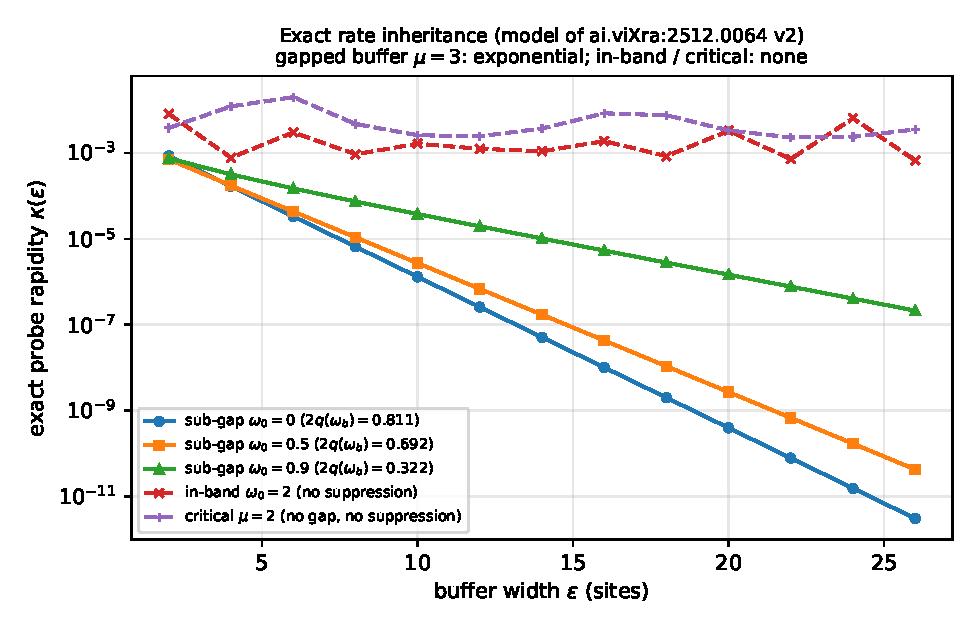
\includegraphics[width=0.82\textwidth]{fig_rip_exact.pdf}
\caption{Exact rate inheritance and its boundaries, from the solvable model
of \cite{HCut} (v2) (probe--Kitaev-buffer--local-sink; exact Liouvillian
rapidities). Sub-gap probes: exponential suppression with the analytic
frequency-resolved slopes $2q(\omega_b)$ shown in the legend. In-band probe
and critical buffer: no suppression. The high-precision four-decimal
fitted-vs-analytic agreement is reported in \cite{HCut}, Table~1, with its
tail-fit protocol; the curves here are the raw exact rapidities. Generated by
\texttt{verification/0072/make\_rip\_figure.py} from the
\texttt{verification/0064} data.}
\label{fig:exact}
\end{figure}

\section{Failure modes}\label{sec:failure}

RIP is not universal. Explicit failure modes:
\begin{enumerate}
\item Critical baths with algebraic correlations
$\langle B(x)B(y)\rangle \sim |x-y|^{-\alpha}$, yielding
$\kappa(\eps) \sim \eps^{-\alpha}$ (and failing the uniform integrability of
Lemma~\ref{lem:weak}).
\item Non-Markovian regimes (the Davies form itself is invalid).
\item Symmetry-protected or cancellation-dominated channels.
\item Nonlocal couplings.
\item \emph{Secular delocalization (new in v2, realized in \cite{Stress}):}
even for strictly local couplings, the finite-size Davies construction
produces delocalized jump operators; near-zero-frequency channels then
sustain rate floors that no geometric separation reduces --- within that
model class. Whether a microscopically local environment reproduces this is
exactly the question the secular limit cannot answer at finite size.
\end{enumerate}

\section{Operational consequences (conditional)}

Assuming the weak-coherence regime (two-sided rate proportionality) and the
maintenance inequality of \cite{MaintWork} (v2) --- which for pure dephasing
holds with no baseline or contraction assumptions --- one obtains for any
$\delta > 0$:
\begin{equation}
C(\rho) \le C_0(\delta) \;\Rightarrow\;
P_{\mathrm{extra}}(\rho) \ge \kB T\, (\kappa(\eps) - \delta)\, C(\rho).
\end{equation}
When rate inheritance holds (quasi-free local-sink class), isolation is
exponentially cheap in $\eps$ and the coherence-lifetime cost is logarithmic
\cite{HCut}; when it fails (persistent floors), one obtains an operational
resource horizon \cite{Stress}. The architectural reading is
\cite{Closure} (v2).

\section{Falsification protocol (proxy-validated)}

RIP (weak form, as an empirical claim about a platform) is falsified if
static correlations decay exponentially while no constants $A, \beta > 0$
exist such that $\kappa(\eps) \le A\,\mathrm{poly}(m\eps)\,e^{-\beta m\eps}$
holds uniformly in a validated gapped Markovian regime --- \emph{provided the
rate is extracted by a validated protocol}: Liouvillian spectra or
fixed-absolute-time exponential fits, with a gap-removed (critical) control
and a dissipation-free baseline, never co-moving windows
\cite{HCut}; and with declared operator subspaces if spectral envelopes are
used \cite{Stress}. v1's protocol lacked the proxy-validation clause; the
series' own history shows it is not optional.

\section{Conclusion}

RIP isolates the dynamical bridge between static clustering and decoherence
rates. Its weak form is a lemma under explicit hypotheses; its strong form is
now derived --- with the squared-amplitude, frequency-resolved exponent ---
in an exactly solvable quasi-free local-sink class, fails through
near-zero-frequency channels within the secular Davies class, and remains
open precisely for interacting gapped buffers with local dissipation.
Combined with the corrected maintenance-power bounds, RIP where valid makes
the quantum--classical transition an engineering statement: isolation is
exponentially cheap in buffer width, and where RIP fails, coherence has an
unavoidable power floor --- a resource boundary either way.

\appendix

\section{Changes relative to version 1}

\begin{enumerate}
\item \textbf{Surrogate evidence withdrawn} (Remark~\ref{rem:withdrawal}):
v1's decay-curve proxy table and its broken figure placeholder
(\texttt{nedladdning.png}, v1's compile-time remark) are replaced by exact
Liouvillian-rapidity evidence (Fig.~\ref{fig:exact}) generated by a
distributed script from the \cite{HCut} verification data.
\item \textbf{Weak form promoted to Lemma~\ref{lem:weak}} with its
hypotheses explicit; the ceiling nature of $\kappa(\eps)$ is flagged
(Remark~\ref{rem:ceiling}).
\item \textbf{Strong form status updated} (Remark~\ref{rem:status}): derived
in the quasi-free local-sink class with exponent $2q(\omega_b)$ --- v1's
squared-envelope caveat, confirmed --- and failure realized within the Davies
class; the interacting-buffer case is delegated to the conjecture of
\cite{HCut}.
\item \textbf{New failure mode} (secular delocalization,
Section~\ref{sec:failure}) and \textbf{proxy-validation clause} in the
falsification protocol.
\item \textbf{Maintenance inequality re-anchored} to \cite{MaintWork} (v2)
(v1 cited the v1 form, whose extra-power definition was vacuous); references
updated to the v2 series with repository paths; \cite{Stress} and
\cite{Closure} added (absent from v1); the author-profile pointer replaced by
the companion repository.
\end{enumerate}

\begin{thebibliography}{9}\small

\bibitem{Clustering} L.~Eriksson, \emph{Clustering, Recovery, and Locality in
Algebraic Quantum Field Theory: Quantitative Bounds via Split Inclusions and
Modular Theory}, ai.viXra:2512.0060, v2 (2026; v1: 2025). Companion
repository, \texttt{papers/0060-clustering-recovery}.

\bibitem{MaintWork} L.~Eriksson, \emph{The Conditional Maintenance Work
Theorem: Operational Power Lower Bounds from Energy Pinching and a
Split-Inclusion Blueprint for Type III AQFT}, ai.viXra:2512.0061, v2 (2026;
v1: 2025). Companion repository, \texttt{papers/0061-maintenance-work}.

\bibitem{HCut} L.~Eriksson, \emph{The Heisenberg Cut as a Resource Boundary:
An Operational Outlook from Coherence Maintenance Costs}, ai.viXra:2512.0064,
v2 (2026; v1: 2025). Companion repository,
\texttt{papers/0064-heisenberg-cut}.

\bibitem{Stress} L.~Eriksson, \emph{Stress Testing the Rate Inheritance
Principle: Spectral Decoherence Rates and an Operational Resource Horizon},
ai.viXra:2512.0070, v2 (2026; v1: 2025). Companion repository,
\texttt{papers/0070-rate-inheritance}.

\bibitem{Closure} L.~Eriksson, \emph{Operational Coherence Maintenance:
Proven Results, Conditional Interfaces, and Open Dynamical Gaps},
ai.viXra:2512.0071, v2 (2026; v1: 2025). Companion repository,
\texttt{papers/0071-program-closure}.

\bibitem{Davies74} E.~B.~Davies, \emph{Markovian master equations}, Commun.
Math. Phys. \textbf{39} (1974), 91--110.

\bibitem{Spohn78} H.~Spohn, \emph{Entropy production for quantum dynamical
semigroups}, J. Math. Phys. \textbf{19} (1978), 1227--1230.

\bibitem{BreuerPetruccione} H.-P.~Breuer and F.~Petruccione, \emph{The Theory
of Open Quantum Systems}, Oxford University Press (2002).

\end{thebibliography}

\end{document}
